\section{Bilgisayar Ağları Modelleme}

\subsection{Simülatör \& Emülatör}

Bilgisayar üzerinde bir ağı modellemek için; simülatör ve emülatör şeklinde iki tür program kullanılmaktadır:

\textbf{Simülatör}: Gerçek ortamdaki sistemler ile (çok benzese de) birebir aynı şekilde çalışmaz. Uçuş simülatörleri buna örnek gösterilebilir. Gerçek sistemlerde kullanılan donanımların üzerindeki yazılımlar bunda kullanılmaz, simülatörlerde kullanılan sanal cihazlarda özel geliştirilmiş ve kısıtlı yazılımlar çalışır. Ayrık zamanda çalışır: gerçek hayatta binlerce saat sürecek bir işlem 1 saniyede yapılabilir;  gerçek hayatta 1ms içerisinde biten bir eylem saniyelerce sürecek şekilde yavaşlatılabilir.

\vskip 0.5cm
\textbf{Emülatör}: Gerçek cihazlarda kullanılan yazılımlar doğrudan burada da çalıştırılır. Virtualbox üzerinde Windows çalıştırmak için, gerçek Windows kurulumu yaptığımızı hatırlayın. Donanımlar sanallaştırılır ama donanımlar üzerinde gerçek yazılımlar (işletim sistemleri) kullanılır. Gerçek zamanda çalışır.

\vskip 0.5cm
Simülatör ve emülatör kavramlarını bilgisayar ağları konusu özelinde özetlemeye çalışalım.
\vskip 0.5cm

İnternet'in ortak dilinin IP olması gibi, bilgisayar ağlarında ortak donanım da Cisco firmasının ürünleridir. Pazara erken girmiş olması, ürünlerinin kaliteli olması, geniş ürün yelpazesi olması, bol miktarda dokümanı olması, kullanıcı sayısının çok olması, vb. nedenlerle bilgisayar ağları çalışan hemen herkes Cisco cihazlara hakim olmaktadır. Bu nedenle, ağ modelleme programlarında öncelikle Cisco cihazlara (yönlendirici, anahtar, vb.) destek sağlanmaktadır.

Emülatör uygulamalarında, \textit{-simülatörlerden farklı olarak-} gerçek Cisco işletim sistemi kullanılması gerekmektedir. Gerçek işletim sistemi kullanıldığı için, gerçek cihazlarla yapılan fiziksel ağ uygulamalarına çok yakın bir çalışma ortamı sağlamaktadır. Bunun en büyük dezavantajı ise Cisco işletim sistemleri ücretli olduğu için ilave maliyet çıkarmasıdır. Diğer taraftan; bu işletim sistemlerinin İnternet'in yeraltı dünyasında yaygınlaşması gibi illegal durumlara da sebebiyet vermektedir.

\subsection{Ağ Modelleme Platformları (Ücretsiz Olanlar)}
\subsubsection*{Cisco Packet Tracer}
Cisco firması tarafından geliştirilmektedir. Cisco'nun Networking Academy adı altında vermiş olduğu eğitimlerde katılımcılara verilmektedir. Bunun haricinde satışı bulunmamaktadır. Simülatör tarzında bir uygulamadır.

\begin{figure}[h]
    \centering
    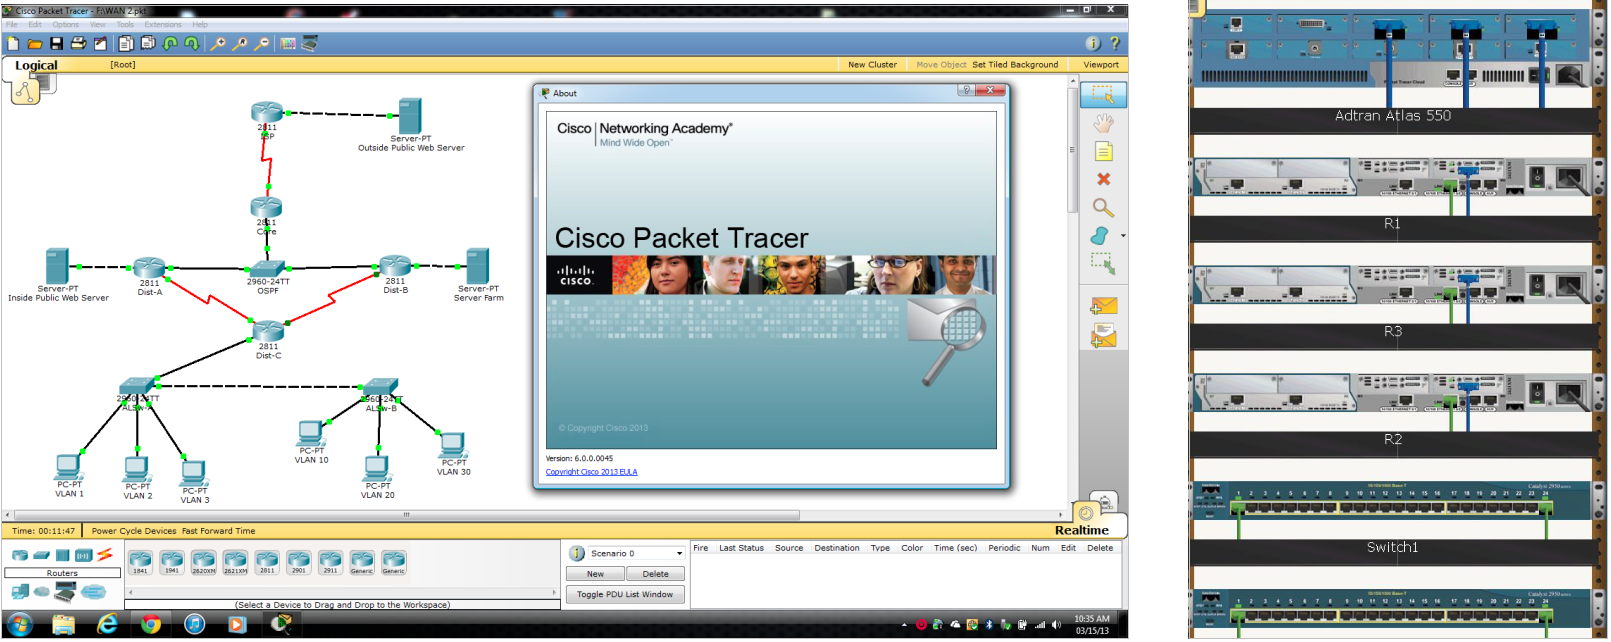
\includegraphics[width=\textwidth]{images/CiscoPT.png}
    \caption{Cisco Packet Tracer arayüzü. Sol tarafta "mantıksal", sağ tarafta "fiziksel" görünüm}
    \label{fig:CiscoPT}
\end{figure}

.